\chapter{Análisis de Variabilidad Conjunta (MEOF)}
\label{chap:meof}

Tras caracterizar por separado la precipitación y el viento en los capítulos previos, este capítulo evalúa su simultaneidad espacio-temporal mediante el Análisis de Funciones Ortogonales Empíricas Multivariadas (MEOF), que integra el viento a 10 metros y la precipitación total para identificar los modos dominantes de variabilidad acoplada.
A diferencia del análisis univariado, la descomposición MEOF expone la geometría del acoplamiento dinámico entre la circulación atmosférica y el campo de precipitación, permitiendo determinar si sus patrones principales covarían en el mismo sector del dominio lagrangiano o responden a dinámicas diferenciadas.

\section{Fraccionamiento de la Varianza Conjunta}
\label{sec:meof_varianza}

La Figura~\ref{fig:all_expvar_meof} presenta el espectro de varianza conjunta explicada por los cinco primeros modos multivariados (MEOF1 a MEOF5), contrastando la Población Global (panel a) con el subconjunto de alta vorticidad (p90, panel b) para las combinaciones de región de ciclogénesis (SBR, LPB, ARG) y fase evolutiva.
Esta figura se obtuvo aplicando el MEOF sobre la matriz estandarizada de anomalías conjuntas de ambas variables (Sección~\ref{subsec:eof_multivariado}), con el fin de cuantificar la dimensionalidad del acoplamiento entre viento y precipitación, y establecer si la covarianza se concentra en un patrón dominante o se distribuye entre múltiples modos competitivos.

En la Población Global, el MEOF1 capta entre el 19\% y el 27\% de la varianza conjunta según fase y región, con caída progresiva hacia los modos secundarios.
Este espectro relativamente concentrado, aunque menos dominante que el EOF1 univariado del viento, indica que en los ciclones ordinarios ambas variables covarían de manera moderadamente acoplada en un único patrón espacial de gran escala, coherente con la organización frontal del WCB que estructura simultáneamente la banda de precipitación y el gradiente de viento en el flanco cálido del sistema.
En el subconjunto de alta vorticidad (p90), en cambio, la varianza explicada por el MEOF1 cae significativamente, con mínimos de 11.65\% en ARG durante la intensificación y 15.41\% en ARG durante la madurez.
Esta reducción y el aplanamiento del espectro hacia los modos secundarios son la manifestación matemática de la \textit{fragmentación de mesoescala}. Cuando los sistemas alcanzan tasas elevadas de intensificación, desarrollan múltiples configuraciones de acoplamiento que compiten en importancia, la aceleración de la CCB frente a las bandas convectivas del sector cálido, la intrusión seca frente al WCB, y ningún patrón único captura más de una fracción minoritaria de la covarianza total, reflejando la mayor complejidad dinámica de los sistemas p90, tal como señalan \citet{hannachi2007empirical} al establecer que un espectro de autovalores aplanado es el indicador estadístico de un sistema complejo y multidimensional.

\begin{figure}[htbp]
    \centering
    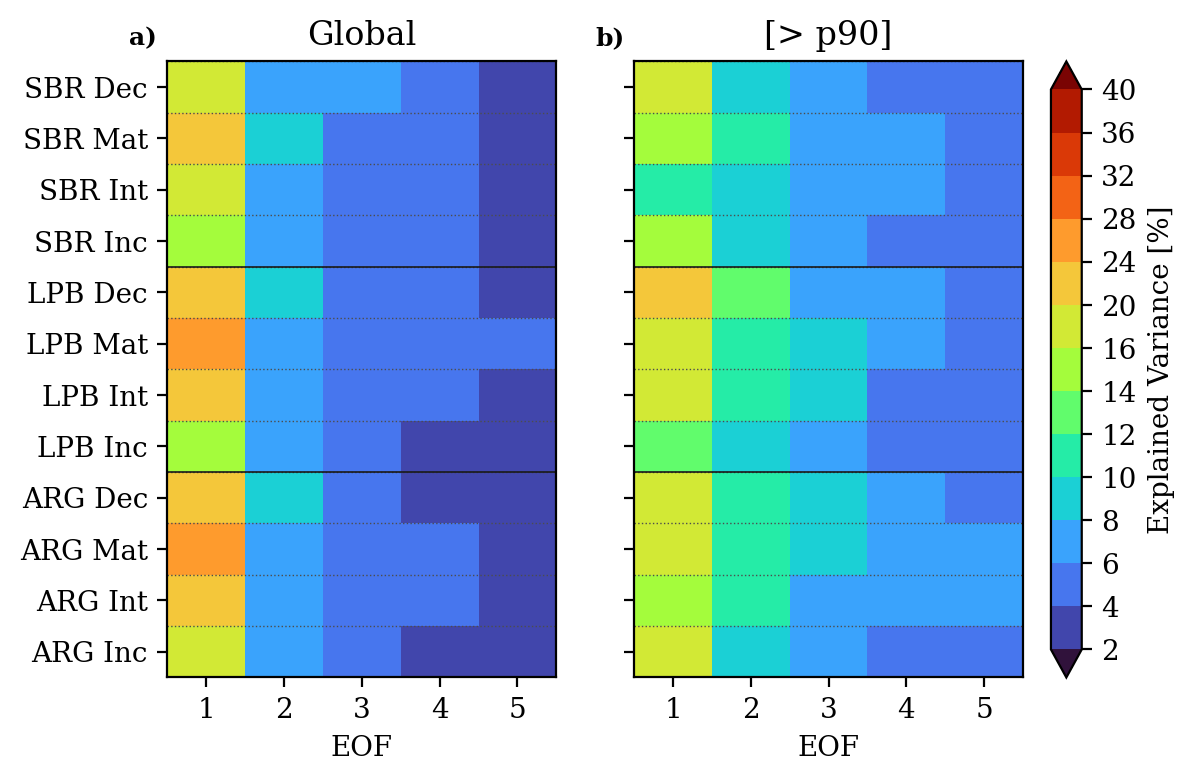
\includegraphics[width=0.8\textwidth]{images/meof/all_expvar_meof.png}
    \caption[Varianza conjunta explicada por los modos acoplados (MEOF1--MEOF5)]{Fraccionamiento de la varianza conjunta total contenida en los primeros cinco modos espaciales multivariados (MEOF1 a MEOF5). Se contrasta la distribución de la covarianza entre el viento a 10 metros y la precipitación para la Población Global (panel a) frente al subconjunto de alta vorticidad (p90, panel b). Las barras de cada fila representan las combinaciones de región de ciclogénesis y fase evolutiva.}
    \label{fig:all_expvar_meof}
\end{figure}

\section{Evolución de los Patrones Espaciales Acoplados (MEOF1)}
\label{sec:meof_patrones}

Los patrones espaciales del primer modo multivariado (MEOF1) revelan cómo se organiza la covarianza de viento y precipitación en el dominio lagrangiano a medida que el ciclón evoluciona.
El análisis se centra en dos fases diagnósticamente centrales: la intensificación, donde se establece la arquitectura de acoplamiento inicial, y la madurez, donde la reorganización espacial entre variables alcanza su expresión más marcada en los sistemas p90.

La selección de estas dos fases, en lugar de las cuatro que componen el ciclo de vida (Sección~\ref{subsec:tb_fases}), obedece a dos razones.
Por un lado, la fase incipiente corresponde por definición a la aparición inicial del núcleo de vorticidad organizada, cuando los sistemas todavía exhiben circulaciones asimétricas antes de consolidar un centro de vorticidad cerrado y presentan una variabilidad de intensidad inter-sistémica marcadamente mayor que en las fases posteriores \citep{reboita2010south}; esta heterogeneidad, ya evidenciada en la baja y dispersa varianza explicada por el EOF1 univariado durante la incipiencia (Secciones~\ref{sec:var_exp_wind10} y~\ref{subsec:var_exp_tp}), refleja que la diversidad de configuraciones responde no solo a la región de ciclogénesis sino a la falta de organización morfológica de los sistemas, lo que limita la interpretabilidad física de un modo acoplado dominante.
Por otro lado, la fase de decaimiento tiene menor relevancia práctica. Los ciclones del Atlántico Sudoccidental desplazan su trayectoria preferencialmente hacia el sureste y el océano abierto \citep{mendes2010climatology, simmonds2000mean}, de modo que en el decaimiento la mayoría de los sistemas ya se encuentra alejada del litoral sudamericano.
Por estas razones, el análisis detallado del MEOF1 se concentra en intensificación y madurez, las fases donde el acoplamiento estructural es estadísticamente más interpretable.

\subsection{Fase de Intensificación}
\label{subsec:meof_intensificacion}

La Figura~\ref{fig:meof_intensificacion_global} presenta el primer modo espacial multivariado (MEOF1) durante la intensificación para la Población Global.
Cada fila corresponde a una región de ciclogénesis (SBR, LPB y ARG) y cada grupo de columnas muestra los patrones acoplados de precipitación (columna izquierda) y viento a 10 metros (columna central), junto con la serie temporal de la componente principal (PC1, columna derecha).
La escala cromática divergente cuantifica las anomalías estandarizadas del MEOF1, con tonos rojos para cargas positivas y azules para negativas en el espacio lagrangiano. La varianza explicada, indicada sobre cada panel de PC1, oscila entre 18.99\% (ARG) y 22.92\% (LPB).
Esta figura se construye aplicando el MEOF sobre la matriz estandarizada de anomalías conjuntas de ambas variables en el dominio lagrangiano centrado en el vórtice, con el fin de establecer el patrón de referencia del desarrollo baroclínico estándar durante el período de intensificación del sistema en la climatología media.

\begin{figure}[htbp]
    \centering
    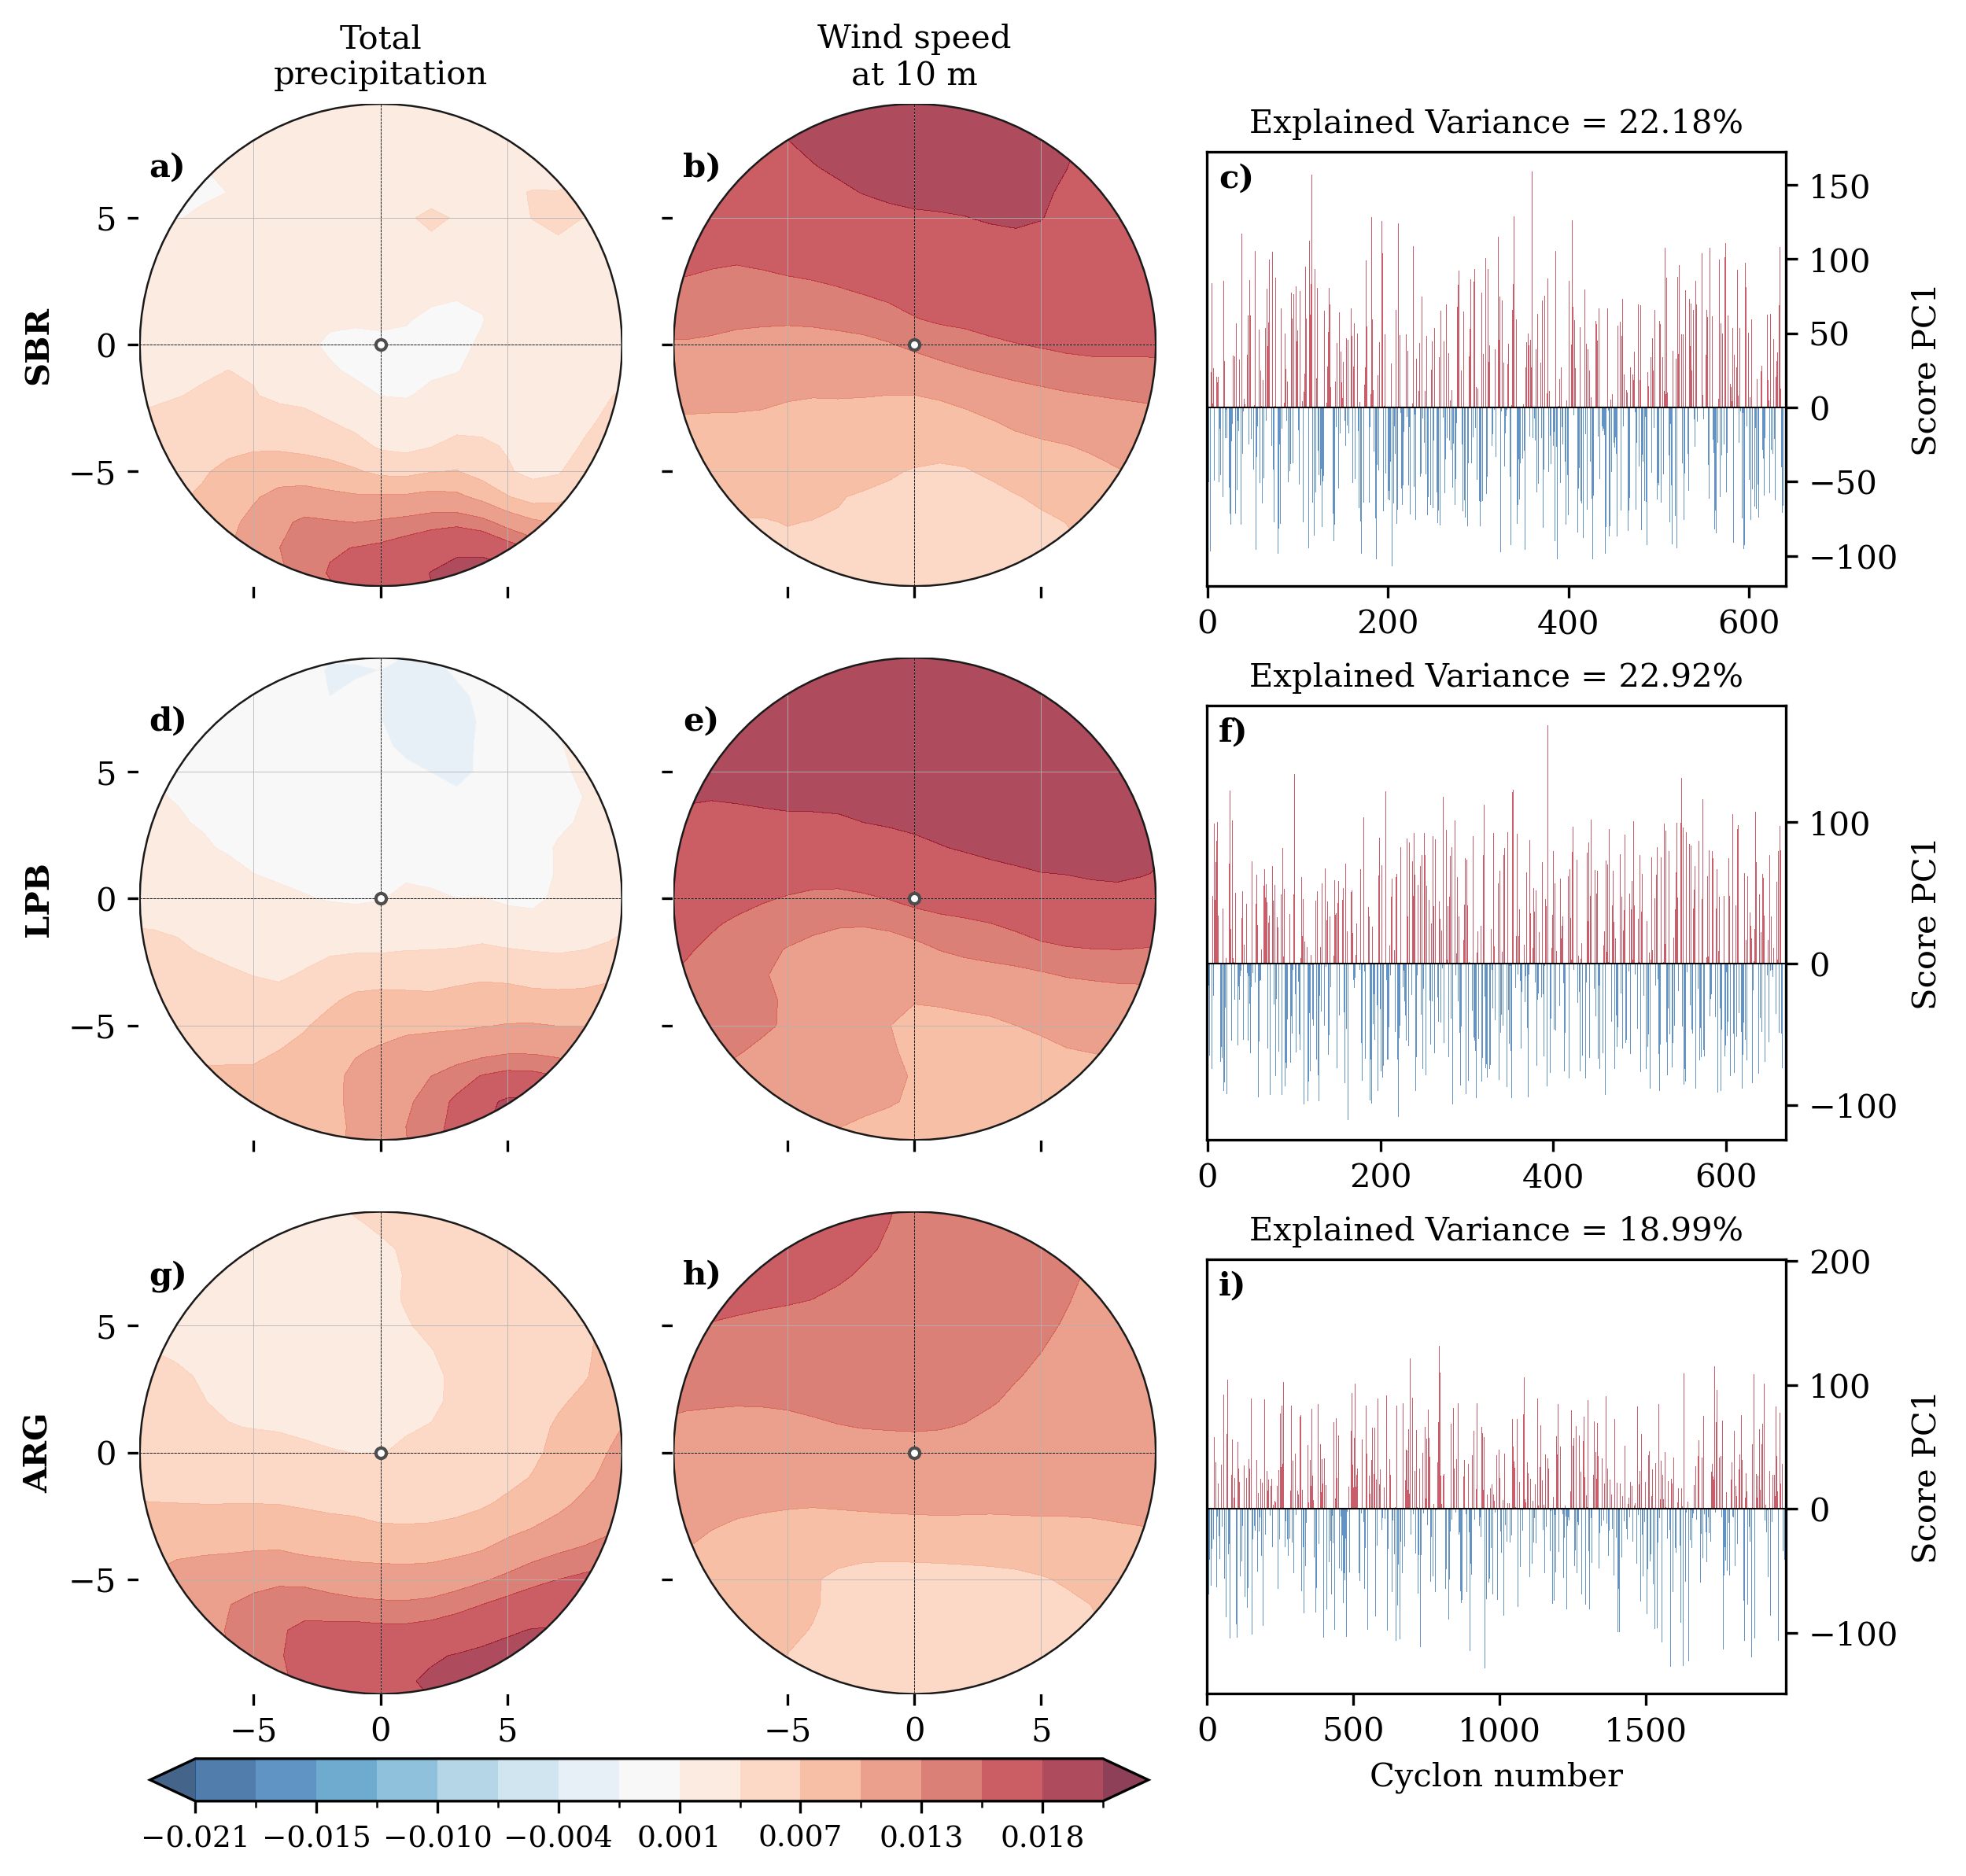
\includegraphics[width=\textwidth]{images/meof/meof1_intensification_global.png}
    \caption[MEOF1 de viento a 10 m y precipitación -- Intensificación (Población Global)]{Primer modo espacial multivariado (MEOF1) durante la fase de intensificación para la Población Global. Las columnas muestran, para cada región (SBR: filas a--c; LPB: filas d--f; ARG: filas g--i), los patrones acoplados de precipitación total (columna izquierda), viento a 10 m (columna central) y la serie temporal de la PC1 (columna derecha). La varianza conjunta explicada se indica sobre cada panel de PC1. La escala cromática divergente cuantifica las anomalías estandarizadas del MEOF1 en el dominio lagrangiano de $20^{\circ} \times 20^{\circ}$.}
    \label{fig:meof_intensificacion_global}
\end{figure}

La Figura~\ref{fig:meof_intensificacion_p90} presenta los mismos patrones del MEOF1 durante la intensificación, restringida al subconjunto de ciclones de alta vorticidad (p90).
Con disposición de paneles idéntica a la figura precedente, su propósito es documentar la primera reorganización estructural del acoplamiento que anticipa la diferenciación espacial completa que se consolidará en la madurez.
La varianza explicada desciende a valores de 11.65\% (ARG), 17.03\% (LPB) y 14.06\% (SBR), reflejando la dispersión de la covarianza hacia modos secundarios.

El contraste con la Población Global es inmediato y profundo. El campo de precipitación (paneles a, d, g) pierde por completo la extensión difusa del patrón global. En SBR (panel a) aparece un núcleo de anomalías positivas intensas y compactas ($>+0.013$) localizado en el cuadrante noreste-este, con un parche de anomalías negativas en el noroeste y sur-suroeste, configurando ya una estructura asimétrica de dos lóbulos diferenciados.
En LPB (panel d), el patrón de precipitación muestra una banda de anomalías positivas orientada de norte a sur en el sector oriental, con anomalías negativas al oeste y suroeste.
En ARG (panel g), el núcleo positivo de precipitación es el más intenso y compacto de los tres, concentrado al noreste y este del vórtice ($\Delta x \approx +1^{\circ}$ a $+3^{\circ}$, $\Delta y \approx 0^{\circ}$ a $+2^{\circ}$), con una carga que alcanza $+0.018$ en el máximo.
El campo de viento (paneles b, e, h) exhibe un comportamiento distinto. En las tres regiones, las anomalías son negativas en casi todo el dominio, con apenas una franja de valores neutros o levemente positivos en el borde noroccidental.
Este patrón, viento predominantemente negativo combinado con precipitación positiva al este, revela ya el germen de la separación de cuadrantes. Los máximos de precipitación y viento no covarían positivamente, sino que el MEOF1 captura una estructura de anticovarianza donde ambas variables se organizan en sectores mutuamente excluyentes.
Las series de PC1 (paneles c, f, i) muestran el efecto directo del tamaño muestral reducido del subconjunto p90. Con entre 60 y 180 ciclones (frente a los 600--1800 del global), aparecen pulsos de amplitud alta y espaciados que superan las amplitudes máximas de la Población Global, reflejando que los eventos individuales de este subconjunto proyectan sobre el modo dominante mucho más intensamente que el promedio climatológico.

\begin{figure}[htbp]
    \centering
    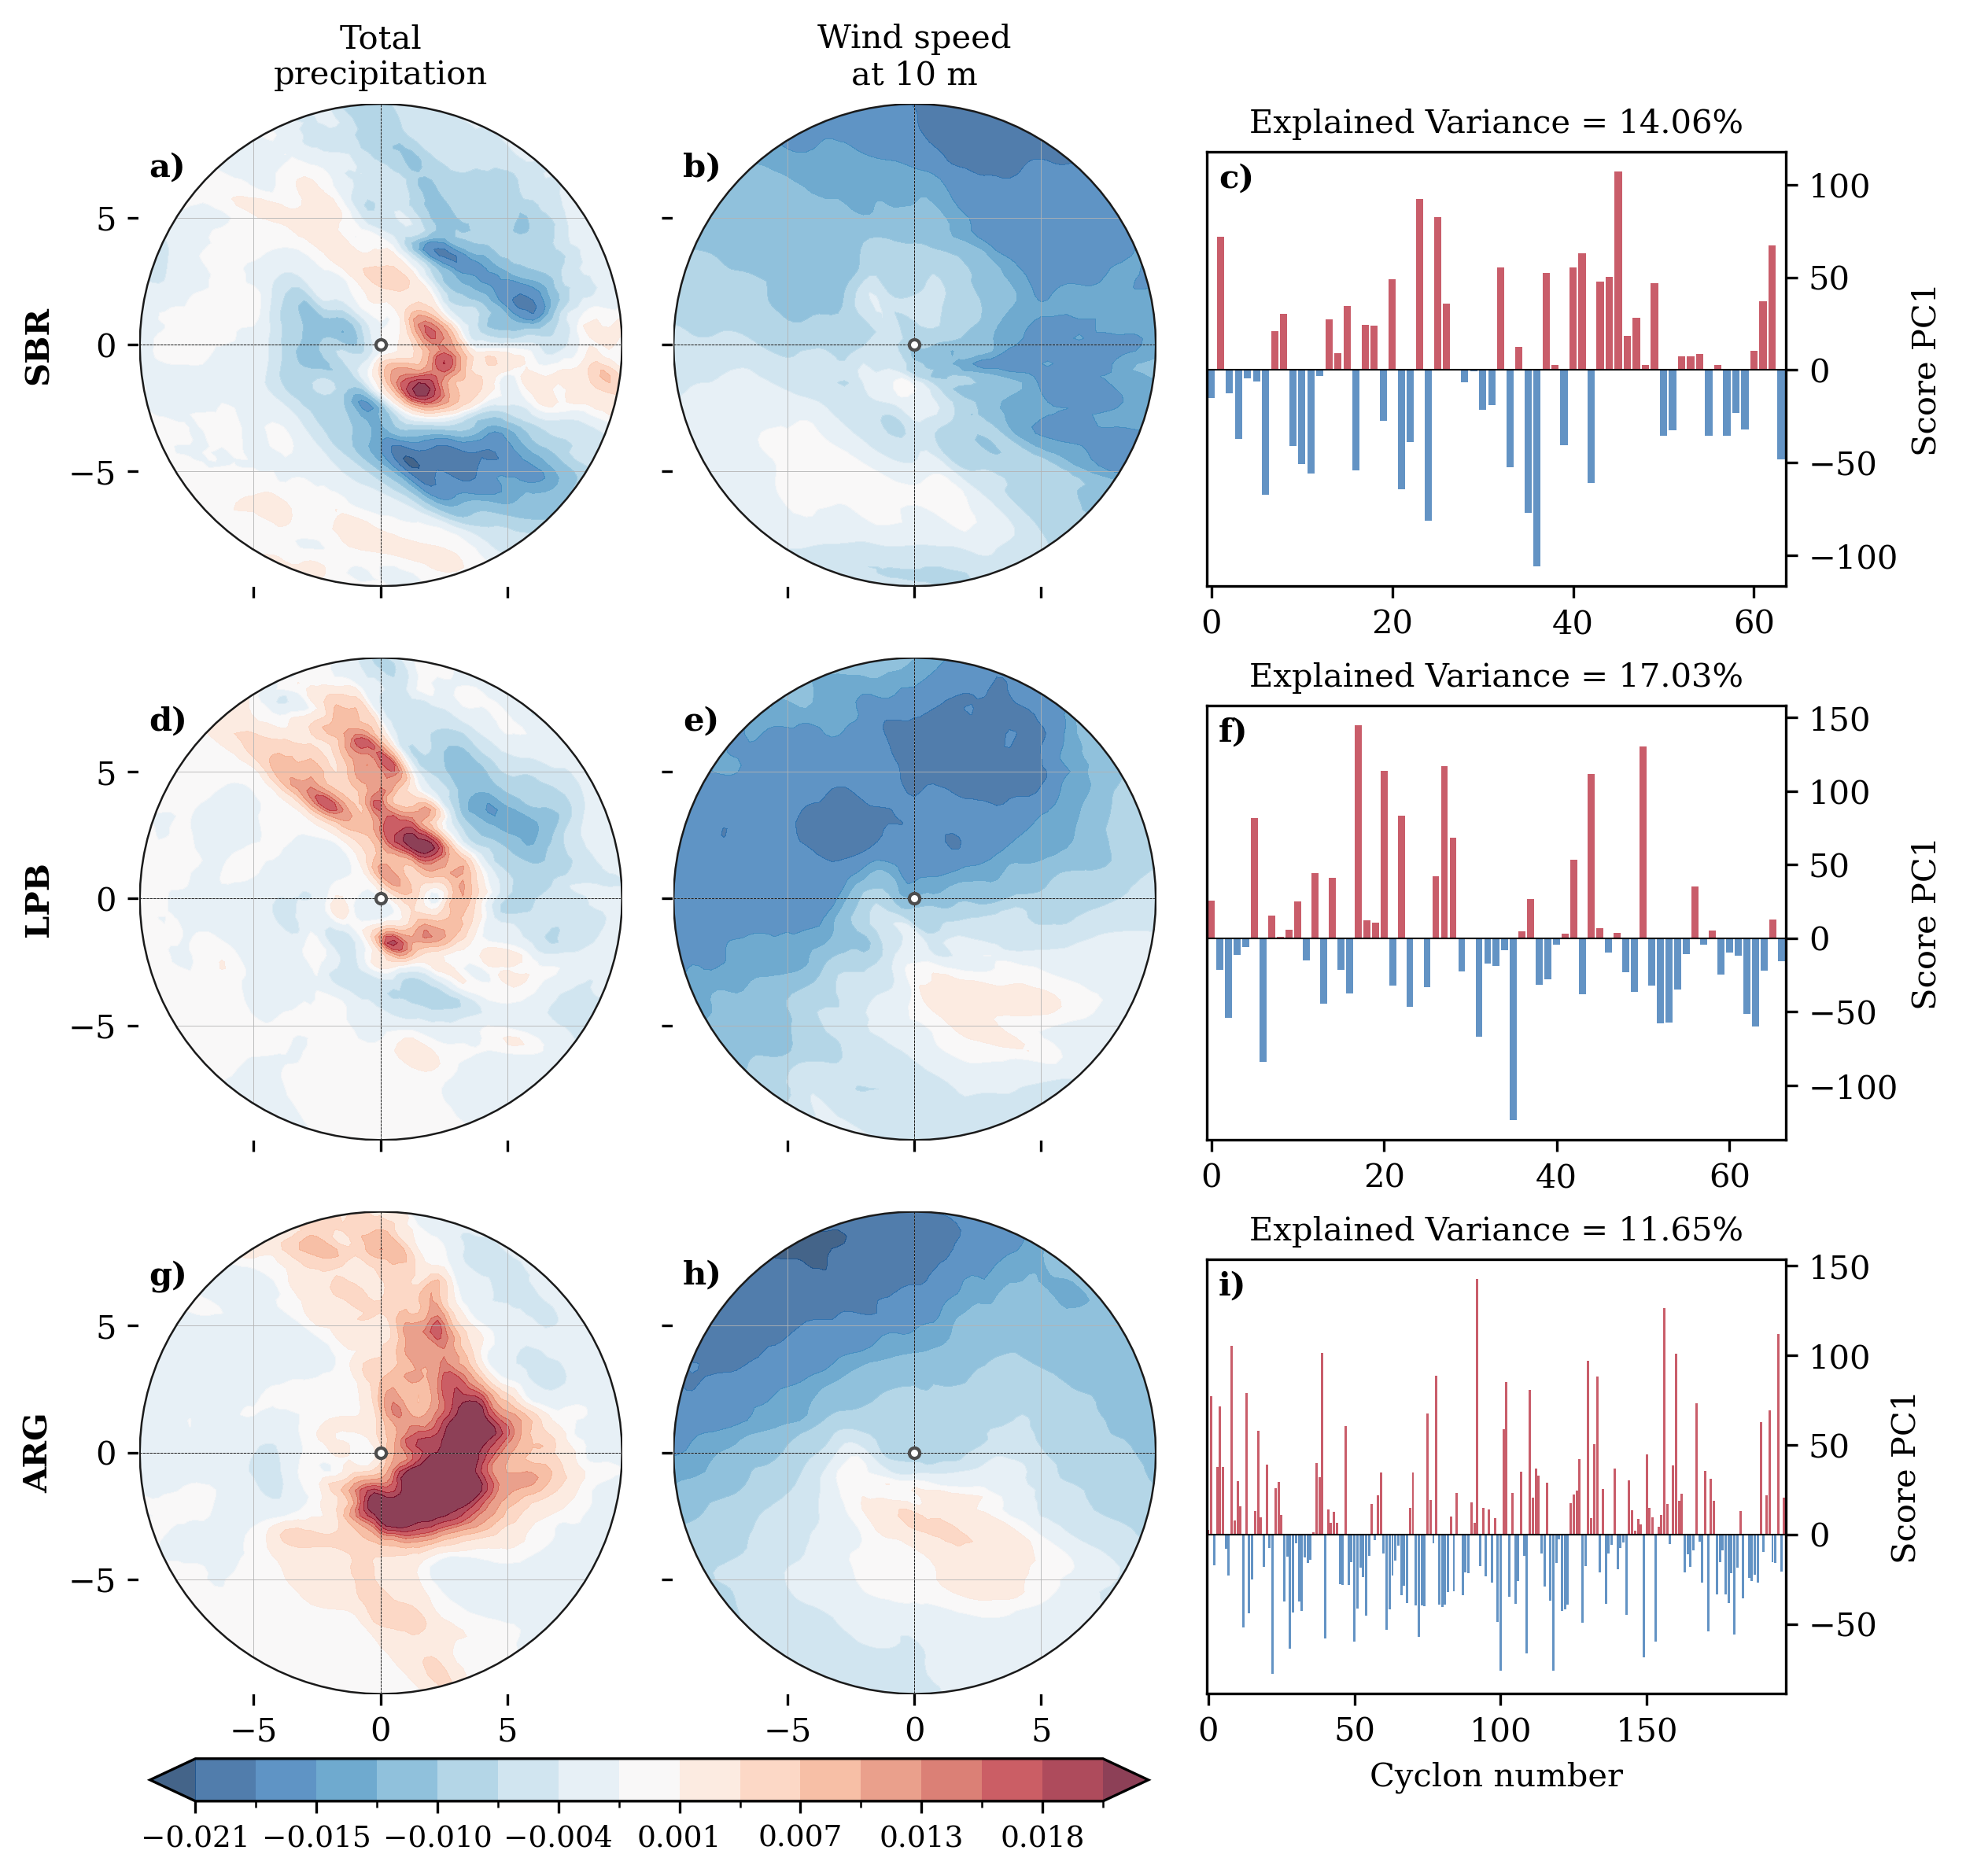
\includegraphics[width=\textwidth]{images/meof/meof1_intensification_p90.png}
    \caption[MEOF1 de viento a 10 m y precipitación -- Intensificación (p90)]{Primer modo espacial multivariado (MEOF1) durante la fase de intensificación para el subconjunto de ciclones de alta vorticidad (p90). El formato de paneles, la escala cromática y el dominio son idénticos a la Figura~\ref{fig:meof_intensificacion_global}, permitiendo cuantificar la contracción de la covarianza y la emergencia de la asimetría estructural durante el desarrollo del sistema.}
    \label{fig:meof_intensificacion_p90}
\end{figure}

La emergencia de la asimetría ya durante la intensificación en los sistemas p90 tiene un fundamento físico preciso.
Durante la intensificación baroclínica activa, la precipitación se organiza en el ascenso frontal del WCB en el flanco cálido-oriental del ciclón, mientras la CCB emergente da forma a la nubosidad de la \textit{cabeza de la coma} \citep{browning1986conceptual} y comienza a envolver el núcleo del sistema.
En ciclones ordinarios, estos dos procesos operan de manera suave y parcialmente superpuesta, generando la covarianza difusa documentada en la Población Global.
En los sistemas intensos, la tasa de intensificación es lo suficientemente elevada como para que la deformación cinemática del vórtice separe físicamente las corrientes ascendentes húmedas de las descendentes frías durante la intensificación misma, antes de que el sistema alcance su máximo.
Esta separación prematura es la razón por la que el MEOF1 ya captura una configuración de anticovarianza en esta fase en los sistemas intensos. La precipitación se concentra al este mientras el viento se intensifica en el sector norte-noroeste, anticipando la configuración opuesta de cuadrantes que dominará en la madurez.

\subsection{Fase de Madurez}
\label{subsec:meof_madurez}

La Figura~\ref{fig:meof_madurez_global} expone el MEOF1 para la fase de madurez en la Población Global, correspondiente al clímax de la vorticidad climatológica del sistema.
Con la misma disposición de paneles por región (SBR, LPB, ARG) y variable (precipitación, viento, PC1), esta figura documenta la máxima organización conjunta que alcanza un ciclón ordinario en su punto de mayor intensidad.
La varianza explicada oscila entre 22.31\% (ARG) y 26.59\% (LPB), los valores más elevados del ciclo de vida en la Población Global.

La característica más notable es que los patrones de precipitación (paneles a, d, g) y viento (paneles b, e, h) exhiben anomalías estandarizadas de signo positivo extensas y de gran escala, aunque concentradas en mitades opuestas del dominio. En las tres regiones, la precipitación presenta cargas positivas en la mitad sur, mientras el viento las presenta en la mitad norte, ambas con gradientes suaves que decaen hacia el sector contrario.
Esta configuración, aunque no constituye una co-localización estricta, refleja el acoplamiento simple y predecible que caracteriza al ciclón ordinario maduro. El gradiente de presión, que fluye de manera continua y organizada alrededor del vórtice, arrastra el campo de viento hacia el flanco delantero mientras el WCB mantiene el suministro de precipitación en el flanco posterior, ambos como manifestaciones del mismo forzante sinóptico de gran escala.
La especificidad regional reside en la magnitud y forma de las cargas: LPB (paneles d--f) muestra la mayor varianza explicada (26.59\%) y las cargas de viento más intensas y uniformes, con valores positivos que cubren prácticamente toda la mitad norte del dominio (panel e); SBR (paneles a--c) exhibe un patrón de precipitación con cargas positivas levemente desplazadas hacia el sur-sureste (panel a); ARG (paneles g--i) muestra la menor varianza explicada (18.99\%) y patrones más difusos, reflejando la mayor variabilidad estructural de los sistemas de esta región.
Las series de PC1 (paneles c, f, i) son las más densas y simétricas del ciclo de vida de la Población Global, con fluctuaciones frecuentes de amplitud moderada que reflejan la diversidad del catálogo, sin que ningún evento individual domine la serie.

\begin{figure}[htbp]
    \centering
    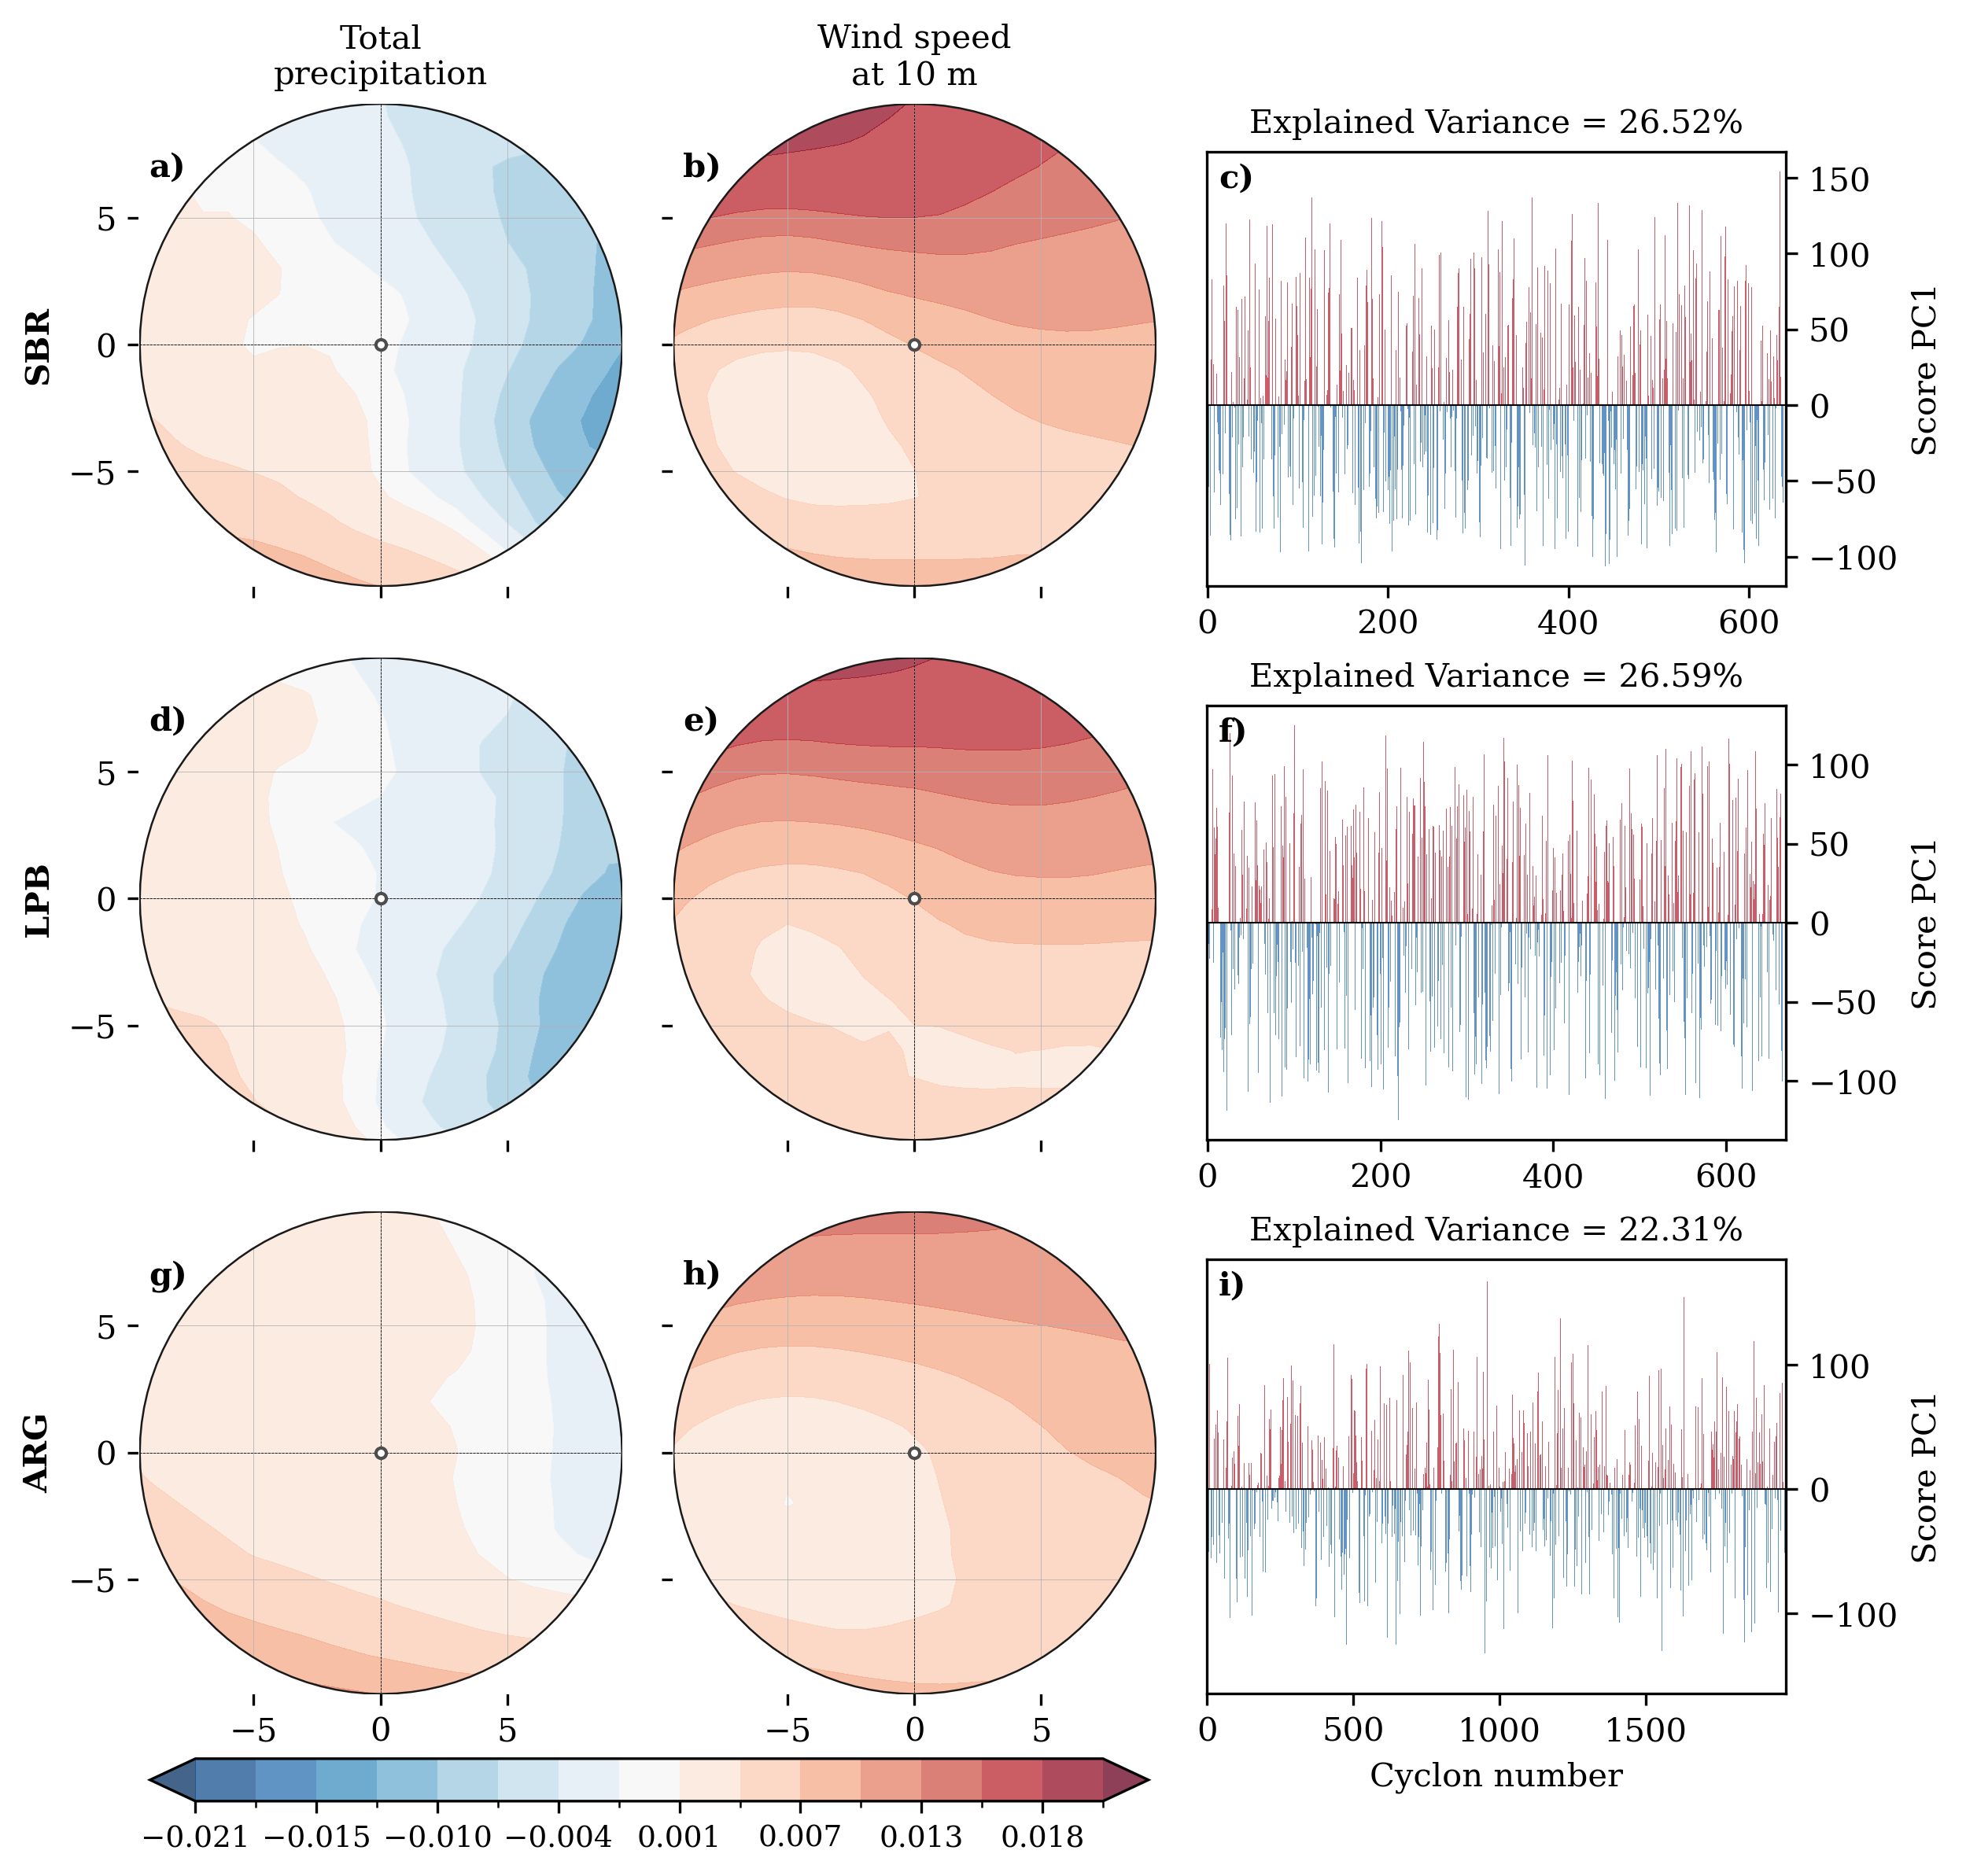
\includegraphics[width=\textwidth]{images/meof/meof1_mature_global.png}
    \caption[MEOF1 de viento a 10 m y precipitación -- Madurez (Población Global)]{Primer modo espacial multivariado (MEOF1) correspondiente a la fase de madurez para la Población Global. La disposición de paneles es idéntica a las figuras precedentes. Se documenta el patrón de acoplamiento de gran escala que caracteriza al ciclón ordinario en su máxima intensidad, estableciendo la línea base respecto a la cual se evalúa la transformación estructural del subconjunto de alta vorticidad.}
    \label{fig:meof_madurez_global}
\end{figure}

La Figura~\ref{fig:meof_madurez_p90} devela la matriz de cargas espaciales del MEOF1 para el subconjunto de alta vorticidad (p90) en la fase de madurez.

Con idéntica disposición de paneles, esta figura constituye el núcleo del capítulo. Su propósito es demostrar la reorganización espacial entre los campos de precipitación y viento en los sistemas p90 del Atlántico Sur. La robustez estadística de esta configuración se apoya en la significancia ya establecida para sus dos componentes univariadas en esta misma fase (Secciones~\ref{subsec:res_significancia_madurez} y~\ref{subsec:significancia_tp}), por lo que no se repite aquí un remuestreo Bootstrap-t multivariado independiente.
La varianza conjunta explicada cae a 15.41\% (ARG), 16.42\% (LPB) y 19.02\% (SBR), muy por debajo de los valores de la Población Global en la misma fase.

El contraste con la figura precedente es el más dramático del capítulo.
El campo de precipitación (paneles a, d, g) exhibe en las tres regiones una estructura arqueada y compacta de anomalías positivas concentrada en el cuadrante sureste y sur del dominio, con un arco enroscado de cargas que alcanzan $+0.018$ en SBR (panel a) y $+0.015$ en LPB (panel d).
Estos valores son los más altos de toda la serie de figuras MEOF, indicando que el modo captura un patrón de precipitación localizado y recurrente en ese sector específico. En SBR, el arco de precipitación (panel a) parte desde el sur y se extiende hacia el este y noreste, trazando la geometría de la banda enroscada (\textit{wrap-around precipitation}) en torno al núcleo del vórtice ocluido.
En LPB (panel d), la banda es más ancha y se extiende desde el cuadrante sur hasta el este, con el pico de carga desplazado hacia el sureste ($\Delta x \approx +3^{\circ}$, $\Delta y \approx -3^{\circ}$). En ARG (panel g), el patrón de precipitación es el más difuso de los tres, con cargas positivas distribuidas en el sureste-sur pero con gradientes más suaves, coherente con la menor intensidad de las oclusiones en esta región.
El campo de viento (paneles b, e, h) presenta una configuración opuesta. Las anomalías positivas se concentran en un núcleo compacto al noroeste del centro, con cargas que alcanzan $+0.013$ en SBR (panel b) y $+0.010$ en LPB (panel e).
Este núcleo de viento noroeste y el arco de precipitación sureste no sólo no comparten sector, sino que en el dominio lagrangiano se ubican en cuadrantes opuestos respecto al centro del vórtice (0,0). Las series de PC1 (paneles c, f, i), con solo 60--65 ciclones por región, muestran pulsos de amplitud extrema que superan con frecuencia el rango $\pm 100$, evidenciando que cada evento individual del subconjunto p90 proyecta una huella muy pronunciada sobre el modo dominante, a diferencia del comportamiento distribuido de la Población Global.

\begin{figure}[htbp]
    \centering
    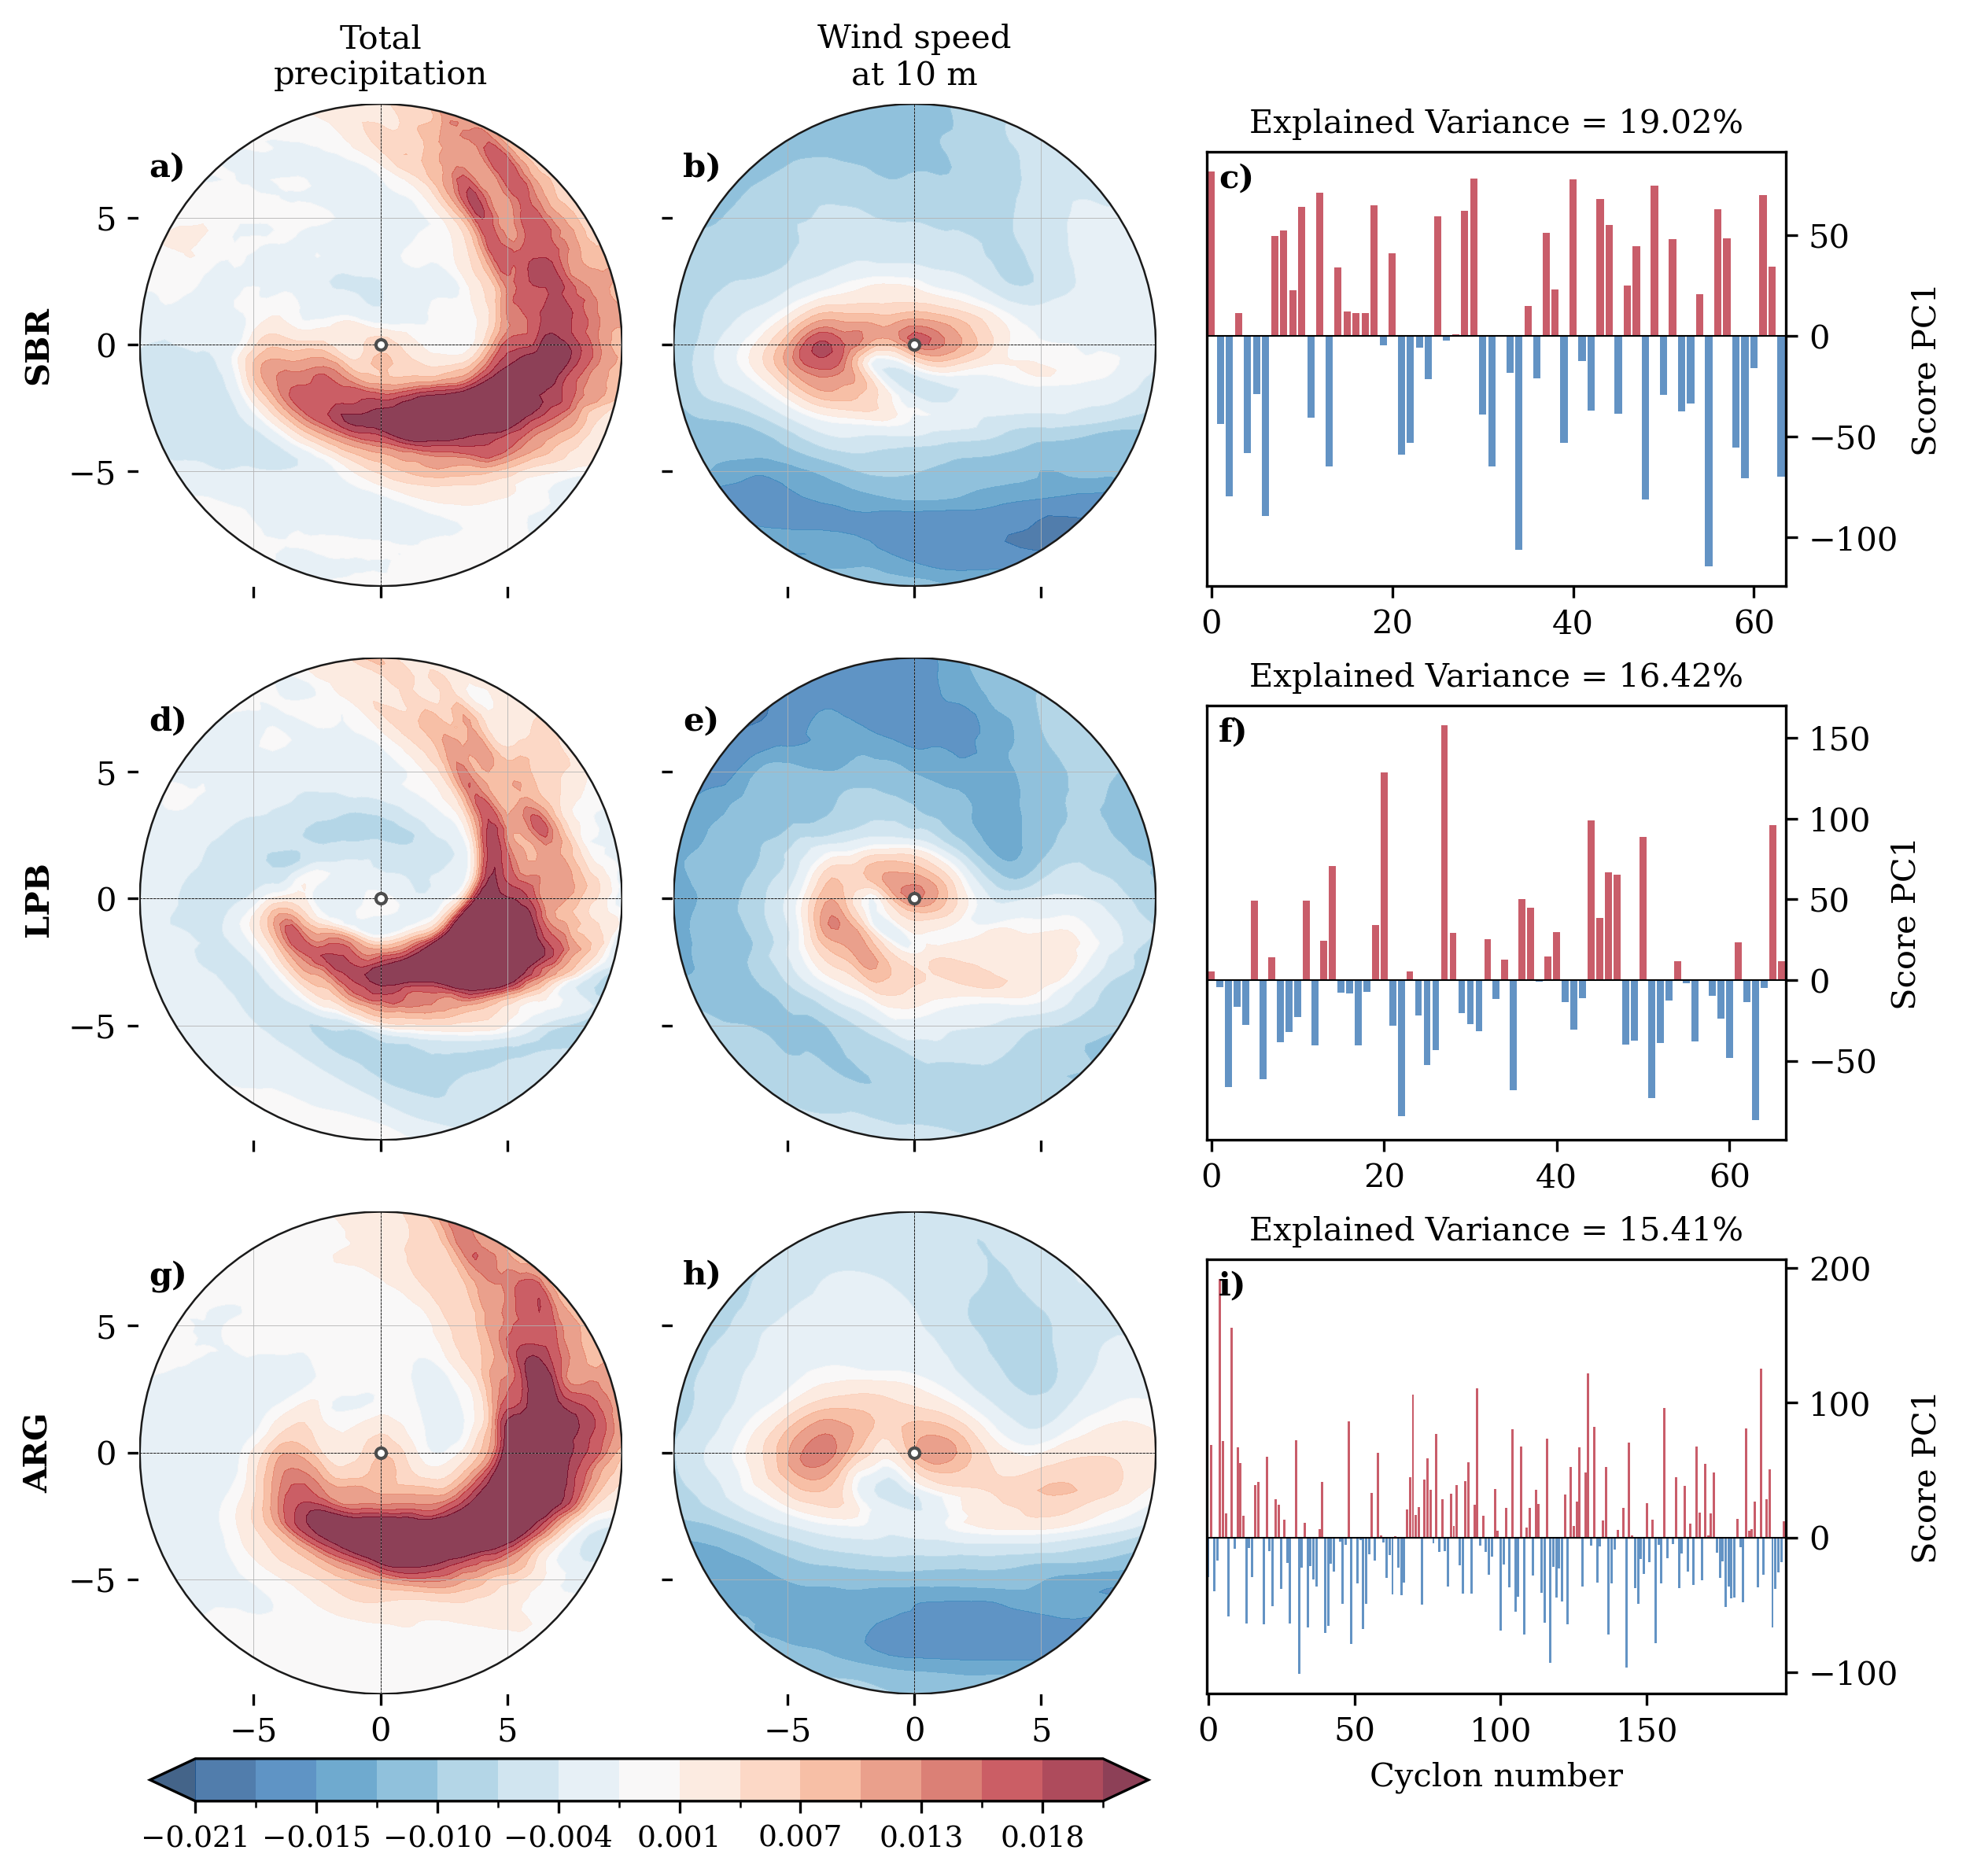
\includegraphics[width=\textwidth]{images/meof/meof1_mature_p90.png}
    \caption[MEOF1 de viento a 10 m y precipitación -- Madurez (p90)]{Primer modo espacial multivariado (MEOF1) correspondiente a la fase de madurez para el subconjunto de ciclones de alta vorticidad (p90). La disposición de paneles, la escala cromática y el dominio son idénticos a las figuras precedentes.
Se evidencia la reorganización espacial entre la banda de precipitación periférica en el cuadrante sureste y el núcleo de viento en el cuadrante noroeste, constituyendo la firma diagnóstica de la estructura ocluida en los sistemas p90 del Atlántico Sur.}
    \label{fig:meof_madurez_p90}
\end{figure}

La configuración de cuadrantes opuestos documentada en el MEOF1 de madurez del subconjunto p90 es la evidencia multivariada que integra y confirma todos los resultados de los capítulos precedentes.
El arco de precipitación sureste capturado por el MEOF1 corresponde a la banda periférica enroscada cuya firma PDFe fue documentada en la Sección~\ref{subsec:kde_tp_p90} y cuyo colapso dimensional fue cuantificado en la varianza del EOF1 univariado (Sección~\ref{subsec:var_exp_tp}).
El núcleo de viento noroeste del MEOF1 replica la concentración espacial identificada en el PDFe de viento p90 (Sección~\ref{sec:kde_espacial_p90}) y la estructura compacta del EOF1 univariado de viento (Sección~\ref{subsec:eof1_wind10_p90}). La novedad que aporta el MEOF es que, al descomponer la covarianza conjunta, demuestra que la separación de cuadrantes no es la yuxtaposición accidental de dos patrones independientes, sino una configuración geométrica estructuralmente coherente. El MEOF1 la captura como un único modo multivariado, lo que confirma que la precipitación sureste y el viento noroeste covarían en los mismos eventos, constituyendo el patrón acoplado dominante de la estructura en el Atlántico Sur.

La interpretación física de esta reorganización espacial es consistente con el modelo de ciclón ocluido de Shapiro-Keyser \citep{schultz2021antecedents}. La intensificación acelerada del sistema se acompaña de aire frío y subsidente que desciende al oeste de su centro, suprimiendo la convección en el núcleo y confinando la humedad residual del WCB a la periferia exterior, consistente con la subsidencia troposférica documentada para el Hemisferio Norte por \citet{shapiro1999bridge}. La separación de cuadrantes documentada valida el marco teórico de la reorganización dinámica del sistema durante la oclusión, donde la cinta transportadora fría (CCB) se consolida en el sector noroeste mientras el WCB residual se reconfigura en la banda periférica sureste.

\section{Coherencia Temporal entre Viento y Precipitación}
\label{sec:meof_coherencia}

Para confirmar si la reorganización espacial observada en los patrones del MEOF1 se traduce también en una divergencia temporal entre los dos campos, se analiza la correlación entre las Componentes Principales univariadas de cada campo ($\text{PC1}^{\text{precip}}$ y $\text{PC1}^{\text{viento}}$), siguiendo la metodología descrita en la Sección~\ref{subsec:analisis_pc}. Los resultados se presentan en la Tabla~\ref{tab:meof_coherencia}, que cuantifica la evolución de este acoplamiento temporal a lo largo del ciclo de vida para ambas poblaciones, con el fin de determinar si la separación espacial de los campos implica también que sus picos de variabilidad ocurren de manera asincrónica dentro del catálogo de ciclones.

\begin{table}[htbp]
\centering
\caption[Coherencia temporal entre precipitación y viento a 10m (Global y p90)]{Correlación de Spearman ($r$) entre la PC1 con signo de precipitación y la PC1 con signo del viento a 10 metros, y su valor de significancia (\textit{p-valor}), para la Población Global y el subconjunto extremo (p90). Los valores en negrita indican correlaciones estadísticamente significativas ($p < 0.05$).}
\label{tab:meof_coherencia}
\begin{tabular*}{\textwidth}{@{\extracolsep{\fill}}llrrrr}
\hline
\textbf{Región} & \textbf{Fase} & \multicolumn{2}{c}{\textbf{Población Global}} & \multicolumn{2}{c}{\textbf{Subconjunto p90}} \\
\cline{3-4} \cline{5-6}
 & & \textbf{$r$} & \textbf{p-valor} & \textbf{$r$} & \textbf{p-valor} \\
\hline
\textbf{SBR} & Incipiente & \textbf{0.31} & $<$ 0.001 & \textbf{0.32} & 0.009 \\
 & Intensificación & \textbf{0.39} & $<$ 0.001 & -0.01 & 0.946 \\
 & Madurez & \textbf{-0.19} & $<$ 0.001 & \textbf{-0.45} & $<$ 0.001 \\
 & Decaimiento & \textbf{-0.19} & $<$ 0.001 & 0.07 & 0.571 \\
\hline
\textbf{LPB} & Incipiente & \textbf{0.25} & $<$ 0.001 & 0.13 & 0.285 \\
 & Intensificación & \textbf{0.35} & $<$ 0.001 & -0.06 & 0.648 \\
 & Madurez & \textbf{-0.08} & 0.029 & \textbf{-0.37} & 0.002 \\
 & Decaimiento & \textbf{-0.08} & 0.032 & 0.12 & 0.314 \\
\hline
\textbf{ARG} & Incipiente & \textbf{0.18} & $<$ 0.001 & 0.03 & 0.647 \\
 & Intensificación & \textbf{0.47} & $<$ 0.001 & -0.08 & 0.236 \\
 & Madurez & \textbf{0.44} & $<$ 0.001 & \textbf{-0.31} & $<$ 0.001 \\
 & Decaimiento & \textbf{0.23} & $<$ 0.001 & \textbf{0.35} & $<$ 0.001 \\
\hline
\end{tabular*}
\end{table}


En la Población Global, las correlaciones entre $\text{PC1}^{\text{precip}}$ y $\text{PC1}^{\text{viento}}$ son positivas durante las fases iniciales en las tres regiones (Tabla~\ref{tab:meof_coherencia}), con valores que oscilan entre $+0.12$ y $+0.40$. En SBR y LPB, esta correlación decae hacia valores cercanos a cero o negativos en la madurez y el decaimiento, coherente con el inicio de la diferenciación entre las trayectorias de ambos campos para los sistemas que comienzan a ocluirse. En ARG, en cambio, el acoplamiento positivo se mantiene significativo hasta la madurez ($\rho = +0.39$) y solo se atenúa en el decaimiento ($\rho = +0.17$), consistente con las oclusiones más graduales y el mayor control orográfico ya documentados en los capítulos previos (Secciones~\ref{sec:pdf_wind10} y~\ref{sec:pdf_tp}).

La incoherencia temporal significativa durante la madurez para los sistemas p90, que alcanza $\rho = -0.49$ en LPB, constituye la evidencia estadística definitiva del \textit{desacoplamiento dinámico}. Un valor de correlación negativo entre las PC1 univariadas de precipitación y viento indica que, dentro del subconjunto de sistemas de alta vorticidad, los ciclones con la proyección más positiva sobre el modo de precipitación (banda enroscada intensa en el sureste) tienden a tener la proyección menos positiva, o negativa, sobre el modo de viento (núcleo noroeste intenso), y viceversa. Esto no implica que las estructuras no coexistan en el mismo ciclón, sino que su organización espacial interna es tal que cuando la banda de precipitación ocupa el cuadrante sureste, el campo de viento se ha reconfigurado hacia el cuadrante noroeste, y la estructura dominante de variabilidad de cada campo opera en sectores distintos del dominio. Estos resultados son consistentes con la reorganización dinámica de la oclusión ya descrita (Sección~\ref{subsec:meof_madurez}). A medida que los ciclones se intensifican, la intrusión seca desacopla la fuente de humedad de la circulación de bajo nivel, maximizando la separación espacial entre los campos de viento y precipitación durante la madurez.

\section{Discusión}
\label{sec:discusion_meof}
% ==============================================================================

Los resultados del análisis MEOF revelan una transición cualitativa en la arquitectura dinámica del acoplamiento viento-precipitación que no es detectable mediante el análisis univariado de cada variable por separado.
En los ciclones de la Población Global, el MEOF1 captura un patrón de covarianza simple y extenso donde viento y precipitación se organizan en el mismo sector del dominio lagrangiano, con una varianza conjunta explicada de entre 19\% y 27\%. Esta configuración refleja el desarrollo baroclínico clásico del modelo noruego de frentes \citep{bjerknes1922life}, sistematizado posteriormente en el marco del WCB como estructura termodinámica única que organiza el ascenso húmedo (precipitación) y el flujo de bajo nivel (viento) en el sector cálido del ciclón \citep{browning1986conceptual}.
La co-localización estadística de las cargas MEOF1 de ambas variables en este sector es la expresión cuantitativa de que, en el régimen medio, los dos campos son manifestaciones del mismo forzante sinóptico y operan como una estructura dinámica acoplada.

La transición al subconjunto p90 introduce un cambio de régimen que no puede atribuirse a una mera amplificación del patrón global.
La caída de la varianza conjunta explicada (de ~26\% a ~15--19\%) y la emergencia de patrones de anticovarianza entre precipitación y viento ya durante la intensificación señalan que los ciclones p90 desarrollan una arquitectura multivariada diferente desde antes de alcanzar su madurez.
Este resultado es coherente con la clasificación de \citet{corner2025classification}, quienes demuestran mediante análisis de componentes principales dispersas que las métricas dinámicas de los ciclones más intensos del Atlántico Norte no escalan linealmente con los parámetros de profundización, sino que exhiben una multidimensionalidad que requiere varias medidas independientes para ser caracterizada.
En el Hemisferio Sur, el MEOF proporciona evidencia equivalente pero en el espacio de la covarianza espacial conjunta. El modo dominante ya no captura un patrón de co-ubicación simple, sino la geometría de separación entre los dos campos dinámicos.

La configuración de cuadrantes opuestos documentada en el MEOF1 de madurez del subconjunto p90 permite, además, establecer una jerarquía física de los procesos involucrados.
El patrón de precipitación enroscada en el cuadrante sureste capturado por el MEOF1 corresponde a la geometría del \textit{trowal airstream}, que \citet{martin1999forcing} describe originalmente como responsable de la banda de precipitación enroscada (\textit{wrap-around precipitation}) en el cuadrante ocluido; la convección embebida en el WCB \citep{oertel2021warm} sostiene además la intensidad pluviométrica localizada en ese sector.
La organización del viento en el cuadrante noroeste es consistente con la caracterización de la CCB como principal motor de la circulación de bajo nivel en la fase de oclusión, que \citet{martinez2014cold} documenta observacionalmente y que \citet{eisenstein2023identification} confirma en climatologías europeas.

Esta configuración acoplada corrobora el vínculo termodinámico subyacente entre ambos flujos; \citet{schemm2014linkage} han demostrado mediante simulaciones que la cinta transportadora fría y el WCB no operan de manera aislada, sino que están conectados dinámicamente mediante la generación de anomalías de vorticidad potencial en la baja y alta troposfera, orquestando el desarrollo integral del ciclón extratropical.
La contribución del MEOF en el presente trabajo es demostrar que estas dos estructuras, documentadas separadamente en la literatura, covarían sistemáticamente en los ciclones p90 del Atlántico Sur. La presencia de la banda enroscada sureste va acompañada de la presencia del núcleo de viento noroeste dentro del mismo evento, constituyendo el prototipo de la estructura ocluida en la región.
Un paralelismo independiente de esta disociación, aunque obtenido con un enfoque de coocurrencia de extremos compuestos en lugar de MEOF, lo aporta \citet{portal2024linking} para el Mediterráneo. Los eventos compuestos de lluvia y viento se maximizan bajo el ascenso del WCB, mientras que los de viento (y oleaje) se maximizan bajo la salida de la intrusión seca, evidenciando en una cuenca de dimensiones y dinámica muy distintas que ambos peligros responden a corrientes en chorro físicamente diferenciadas dentro del mismo ciclón.

Las diferencias regionales en el grado de separación y en la varianza explicada son consistentes con los distintos regímenes termodinámicos documentados en los capítulos previos. En SBR y LPB, la disponibilidad de flujos de calor latente oceánico \citep{gozzo2013air, coutodesouza2024thesis} genera las oclusiones más rápidas, con el mayor desacople geométrico entre las cargas del MEOF1 de precipitación y viento. En ARG, la modulación orográfica y la menor disponibilidad de humedad oceánica producen oclusiones más graduales, con un desacople moderado y cargas MEOF1 de precipitación más difusas.

\section{Síntesis}
\label{sec:sintesis_meof}

El análisis multivariado del MEOF demuestra que los ciclones p90 del Atlántico Sur desarrollan una arquitectura dinámica asimétrica que difiere de la de la Población Global.
Primero, en términos de la dimensionalidad del acoplamiento, mientras que en la Población Global el MEOF1 captura ~20--27\% de la covarianza conjunta con un patrón simple de co-ubicación de ambas variables en el sector frontal oriental, en los sistemas de alta vorticidad (p90) la varianza cae a 12--19\% y se distribuye entre múltiples modos competitivos, expresando la fragmentación de mesoescala que opera cuando la intensificación del vórtice es mayor.
Segundo, en términos de la geometría del acoplamiento, el MEOF1 de madurez del subconjunto p90 captura un patrón de anticovarianza donde la precipitación y el viento se organizan en cuadrantes opuestos del dominio lagrangiano, con el arco de precipitación enroscada al sureste y el núcleo de viento al noroeste, separados por la intrusión seca.
Este hallazgo, respaldado por las correlaciones negativas entre las PC1 univariadas durante la madurez, valida que los sistemas p90 del Atlántico Sur no son la intensificación sincrónica de un único patrón frontal, sino la reorganización estructural de dos campos dinámicos físicamente distintos que operan en sectores diferenciados.
Las bases físicas y estadísticas establecidas en este capítulo sustentan los prototipos estructurales presentados en el Capítulo~\ref{cap:prototipos}, donde la geometría del MEOF1 se integra con las densidades probabilísticas KDE para construir representaciones cuantificadas de la estructura dinámica por región y fase evolutiva.
